% ----------------------------------------------------------------
% Descrição do Trabalho, relevância e abordagens.
% ----------------------------------------------------------------
\chapter{Introdução}
\label{introducao}

\section{Contexto}

Com o crescente mercado de jogos digitais, a demanda por conteúdos novos, cada vez mais sofisticados, diferenciados e muitas vezes personalizados, também aumenta. Infelizmente o custo e escalabilidade para criação manual de novos conteúdos, tão variados, é alta e não escalável. Com isso, muita atenção tem sido dada para técnicas de Geração Procedural de Conteúdo (\emph{Procedural Content Generation} - PCG), tanto no meio comercial quanto acadêmico. PCG é o termo geral para o processo onde métodos algorítmicos são utilizados para geração de conteúdo, seja em jogos ou outros contextos \cite{angelides2014procedural}. O conteúdo gerado pode incluir, mas não se limita a, terrenos, mapas, itens, recompensas, posicionamento de inimigos, distribuição de recursos, áudio, árvores de diálogo, objetivos de missões, padrões de comportamentos, e muitos outros. Estudos recentes, como \cite{hendrikx2013procedural}, \cite{togelius2011search} e \cite{yannakakis2011experience}, avaliam e relacionam diversas metodologias e áreas onde a PCG pode ser aplicada em jogos.

De forma geral, sistemas PCG são desenvolvidos para produzir variação de conteúdo com base em permutações, e como na maioria das vezes se baseiam em aleatoriedade para gerar diversidade e escalabilidade, a não ser que sejam associados a uma semente aleatória específica, cada execução irá gerar um resultado diferente. Isso não só permite aos desenvolvedores criar uma grande variação de modelos e conteúdo, mas também possibilita que jogadores possam vivenciar diferentes desafios e eventos cada vez que jogam um mesmo jogo. De fato, técnicas de PCG são apropriadas para a solução de diversos problemas na área de desenvolvimento de jogos \cite{angelides2014procedural}.

São elas:

\vspace{-5mm}
\begin{itemize}[leftmargin=1.25\parindent]
    \item \textbf{Restrições de memória:} Embora tenha ganho muito mais atenção e visibilidade nos últimos tempos, várias técnicas de PCG vêm sendo utilizadas desde a década de 80 em jogos como \emph{Rogue} \cite{game:rogue} (Figura \ref{fig:game_rogue}), \emph{River Raid} \cite{game:riverraid}, \emph{Pitfall!} \cite{game:pitfall} e \emph{Elite} \cite{game:elite}, por contribuir com soluções de problemas como restrições de memória e armazenamento \cite{aycock2016procedural}. Ainda que este problema possa ser encontrado em consoles portáteis e jogos de celular nos dias de hoje, a popularidade dos métodos de PCG atualmente se deve à outras adversidades, relacionadas à crescente complexidade em geração de novos conteúdos, que também podem ser resolvidas através de seu uso.
    
    \begin{figure}[htb]
    	\begin{center}
    		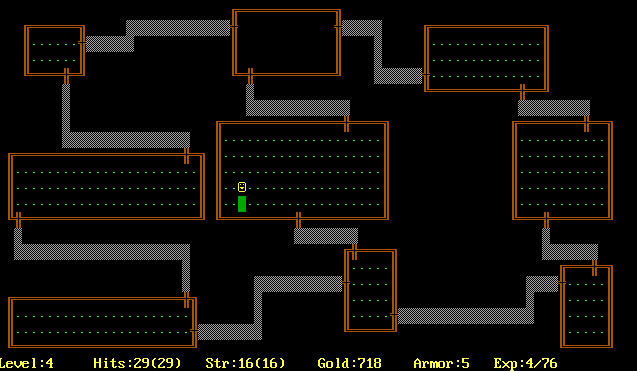
\includegraphics[width=0.75\textwidth]{Imagens/game_rogue.png}
    		\caption{Captura de tela do jogo \emph{Rogue} \cite{game:rogue}. Um dos primeiros jogos a criar mapas de forma procedural, predecessor que deu nome ao gênero de jogos conhecidos como \emph{roguelike}.}
    		\label{fig:game_rogue}
    	\end{center}
    \end{figure}
    
    \item \textbf{Demanda por maior nível de detalhes:} Com jogos tendo mundos cada vez mais imersivos e complexos, a exigência por nível de detalhes e interação por parte dos jogadores aumenta de forma drástica. A criação manual de detalhes como folhas, rochas e outros artefatos em um mundo virtual complexo como os de jogos de hoje em dia é impraticável. O jogo \emph{Left 4 Dead} \cite{game:left4dead}, por exemplo, utiliza técnicas de PCG para geração de zumbis diferenciados utilizando permutações de partes de modelos como cabeças, tórax e braços de forma inteligente com base nos cenários.
    \item \textbf{Longevidade e valor de repetição (\emph{replay value}):} Com a finalidade de aumentar a quantidade de conteúdo oferecida aos jogadores, e sem a necessidade de criar novos conteúdos manualmente. Alguns jogos como \emph{Diablo} \cite{game:diablo} (Figura \ref{fig:game_diablo}), por exemplo, utilizam as características aleatórias da PCG para geração de itens e terrenos, fazendo com que jogadores retornem a jogá-lo somente pela possibilidade de encontrar novos itens ou locais para suas aventuras. Em jogos como \emph{Minecraft} \cite{game:minecraft} e \emph{Terraria} \cite{game:terraria}, por exemplo, a exploração de conteúdo gerado aleatoriamente, com base em elementos já conhecidos, é a principal mecânica do jogo.
    
    \begin{figure}[htb]
    	\begin{center}
    		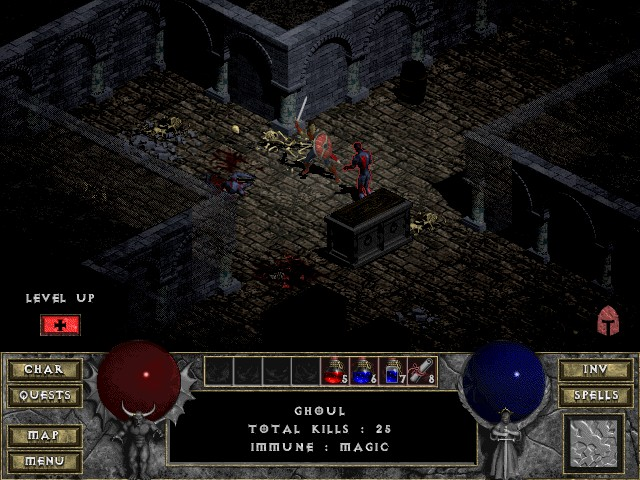
\includegraphics[width=0.75\textwidth]{Imagens/game_diablo.jpg}
    		\caption{Captura de tela do jogo \emph{Diablo} \cite{game:diablo}. Os jogos da franquia utilizam técnicas de PCG para criar itens e mapas, fazendo com que jogadores retornem ao jogo pela possibilidade de encontrar melhores itens para seus personagens.}
    		\label{fig:game_diablo}
    	\end{center}
    \end{figure}
    
    \item \textbf{Novidade e inovação:} Também devido aos padrões de aleatoriedade oferecidos pela PCG, uma característica interessante emergente é a possibilidade de encontrar combinações inovadoras e inesperadas de conteúdo; estas que muitas vezes são capazes de surpreender até mesmo os próprios desenvolvedores. Enquanto em sistemas lineares a utilização de árvores de decisão pode aumentar a variabilidade das experiências dos jogadores, o custo para produção de diversas experiências também é crescente. A imprevisibilidade provida pela PCG oferece aos jogadores o senso de que cada mundo gerado é único e existe para um propósito próprio.
    \item \textbf{Propriedade e autoria:} Provavelmente uma consequência do item anterior, os jogadores sentem que, devido ao conteúdo único e diferenciado, a narrativa dos eventos ocorridos durante jogos com PCG se torna algo mais pessoal. Especialmente em jogos como \emph{Minecraft} \cite{game:minecraft} (Figura \ref{fig:game_minecraft}), \emph{Terraria} \cite{game:terraria} e \emph{Spore} \cite{game:spore}, a combinação de conteúdos únicos gerados pela PCG, em adição ao criado pelos próprios jogadores, oferece um forte senso de propriedade e autoria, engajando ainda mais o jogador ao mundo sendo desenvolvido.
    
    \begin{figure}[htb]
    	\begin{center}
    		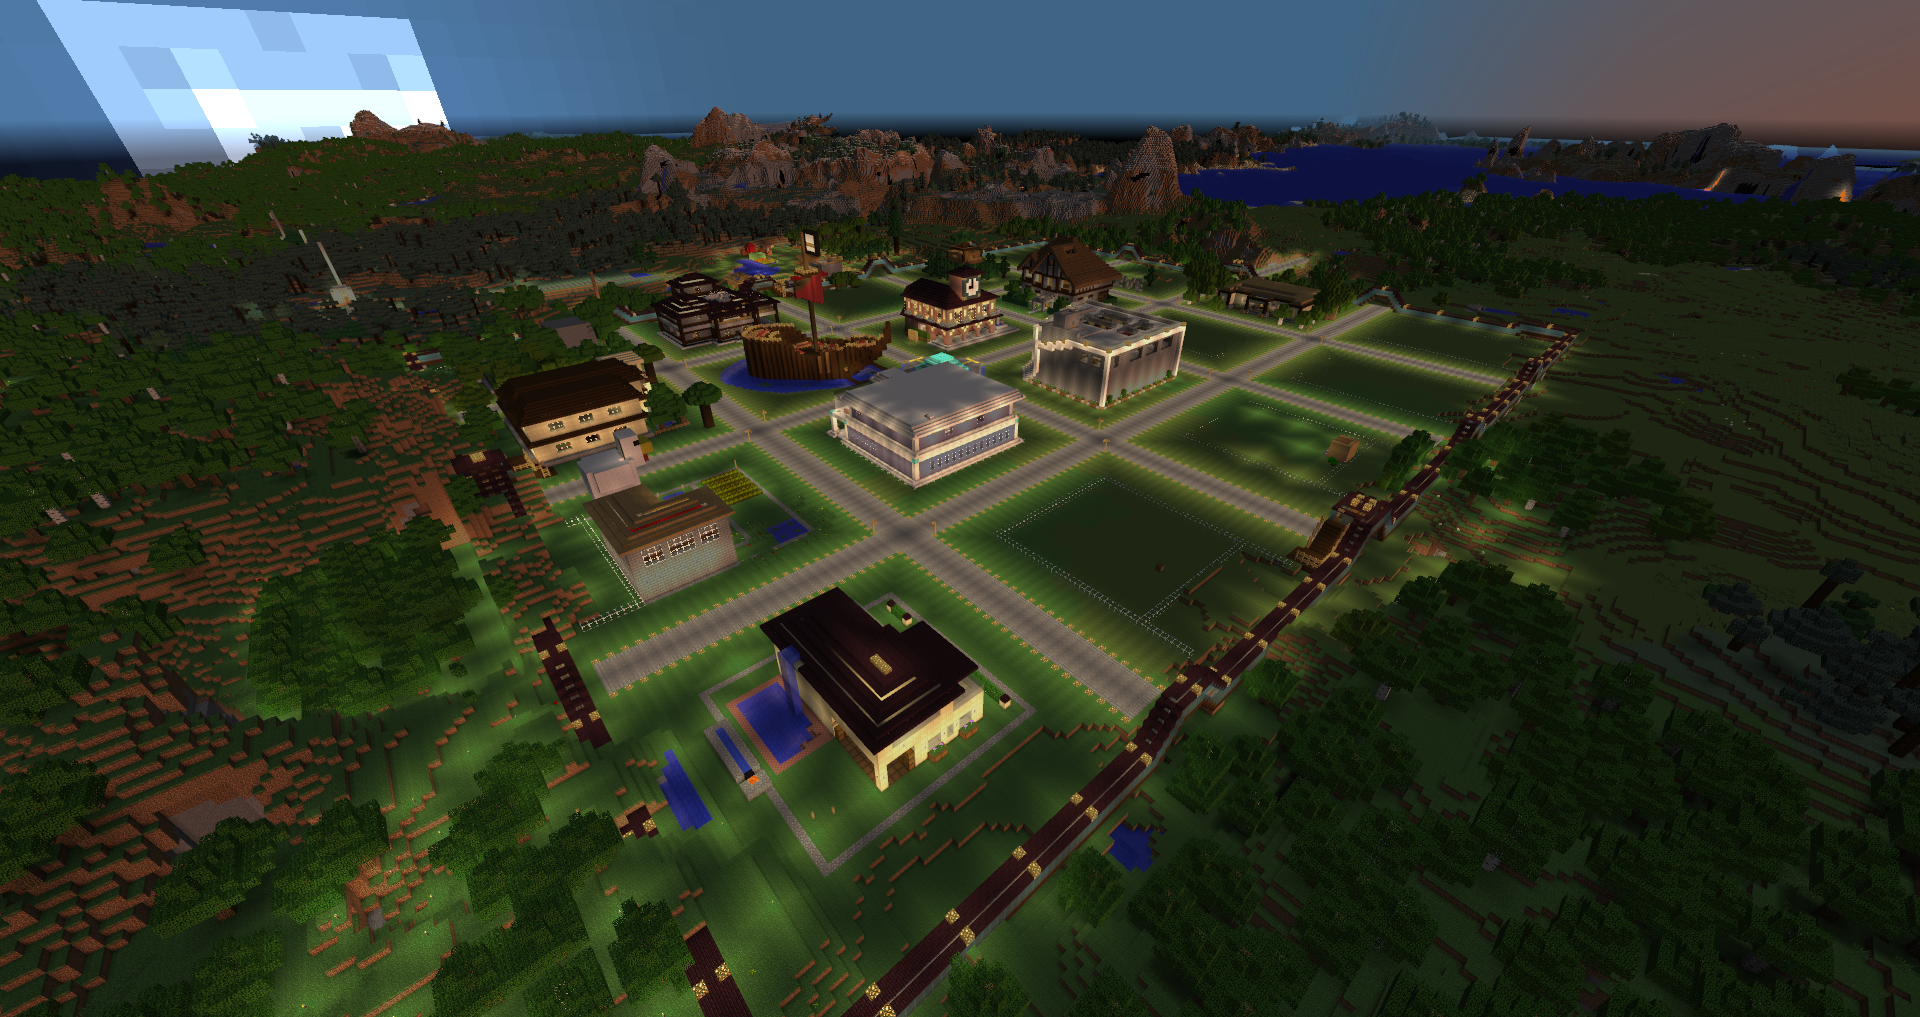
\includegraphics[width=0.8\textwidth]{Imagens/game_minecraft.png}
    		\caption{Captura de tela do jogo \emph{Minecraft} \cite{game:minecraft}. Cidade criada por jogadores em um mundo gerado completamente de forma procedural. Esta combinação é uma excelente fómula para criar um senso de propriedade e autoria em seus jogadores.}
    		\label{fig:game_minecraft}
    	\end{center}
    \end{figure}
    
\end{itemize}

É importante notar também, que técnicas de PCG podem ser executadas em modo \emph{offline}, \emph{online}, ou até mesmo como uma combinação de ambos. Conforme definido em \cite{togelius2011search}, o termo \emph{offline} PCG se refere a geração de conteúdo durante a fase de desenvolvimento da aplicação e, de forma geral, uma vez criado e publicado, o conteúdo nunca se altera; em contrapartida, \emph{online} PCG descreve uma forma mais “ativa” de geração de conteúdo, sendo aplicada durante a execução do programa. A última, frequentemente envolve a geração de conteúdo apoiado por regras baseadas em estados atuais da aplicação ou usuário. Como forma de combinação entre as duas técnicas, podemos ter mapas imutáveis em um jogo que tenham sido criados de forma \emph{offline}, e então usar técnicas \emph{online} para população e variação de itens e inimigos no mapa. Outra forma possível para a combinação de ambos é em uma aplicação que ofereça conteúdo diversificado diariamente, com base em estatísticas e dados recolhidos do usuário nos últimos dias.

A técnica de \emph{offline} PCG pode ser considerada como uma forma de auxílio à tomada de decisões, sendo utilizada para gerar esboços de conteúdos que serão refinados pelos desenvolvedores em etapas seguintes. Outra forma de utilização de \emph{offline} PCG, é justamente para o auxílio a criação de detalhamento e diversidade durante o processo de refinamento de conteúdo, gerando automaticamente vegetação, construções, personagens, entre outros, de forma abrangente e eficiente. Como exemplo de \emph{offline} PCG, o jogo \emph{Oblivion} \cite{game:oblivion} (Figura \ref{fig:game_oblivion}) utilizou de um sistema PCG assistido para a geração da maioria de seus terrenos e florestas.

\begin{figure}[htb]
	\begin{center}
		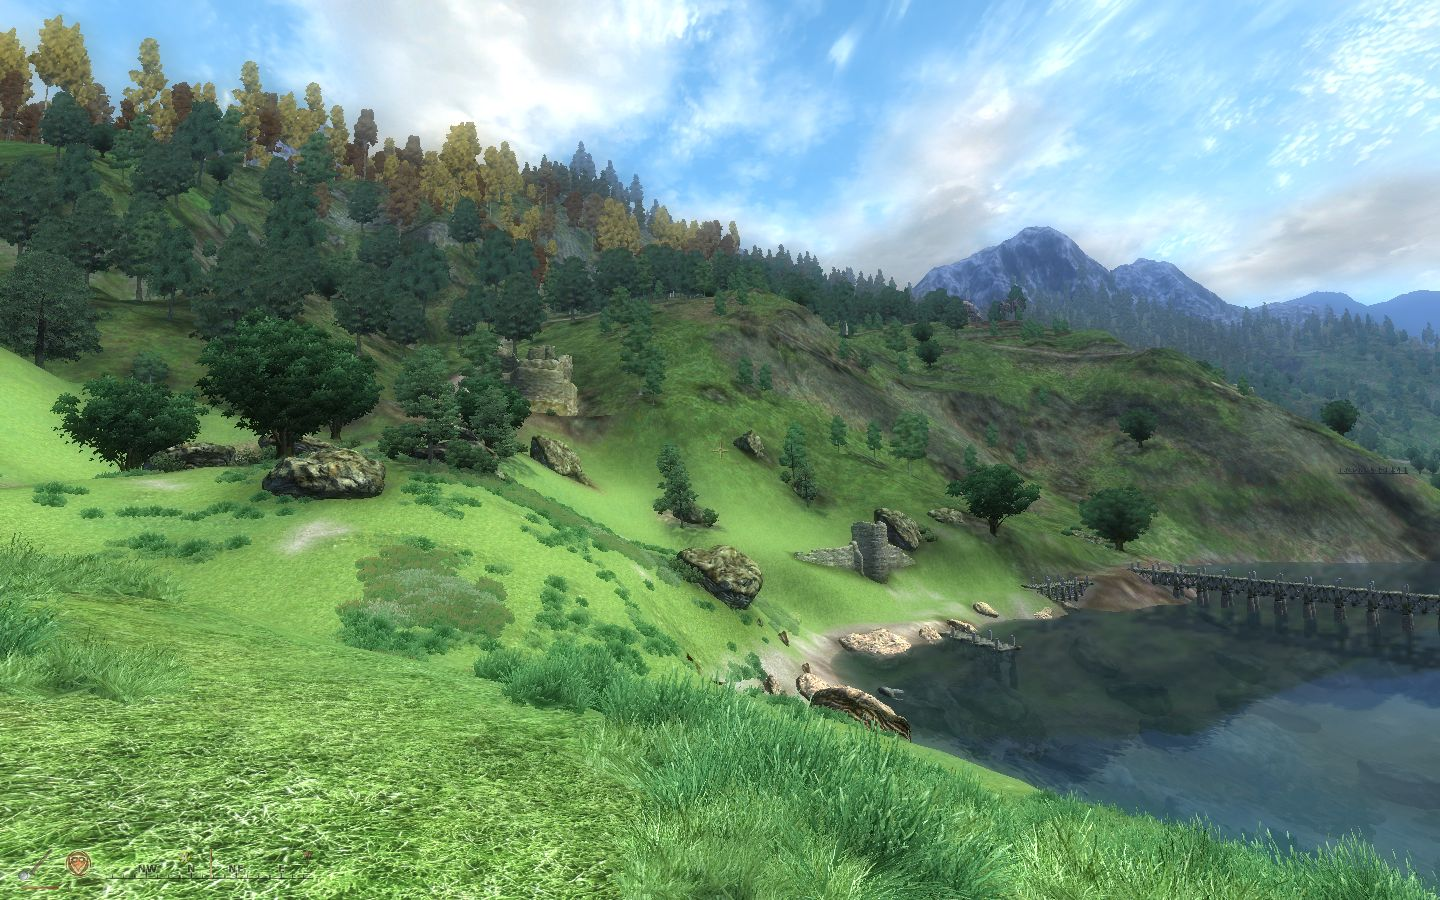
\includegraphics[width=0.8\textwidth]{Imagens/game_oblivion.jpg}
		\caption{Captura de tela do jogo \emph{Oblivion} \cite{game:oblivion}. Tecnicas de \emph{offline} PCG foram utilizadas para geração da maioria de seus terrenos e florestas.}
		\label{fig:game_oblivion}
	\end{center}
\end{figure}

\emph{Online} PCG em geral ocorre de forma mais reativa que sua contraparte, gerando uma relação interativa contínua com o atual estado do jogo. Esta modalidade de PCG é mais complexa em termos de definição e planejamento, uma vez que sua utilização permite que o mundo do jogo e suas mecânicas mantenham evoluções e mudanças constantes e de forma autônoma. Por este motivo, conteúdos gerados desta forma acabam influenciando as dinâmicas de jogo e muitas vezes o nível de dificuldade dos desafios enfrentados pelo jogador. O jogo \emph{Borderlands} \cite{game:borderlands} (Figura \ref{fig:game_borderlands}) utiliza \emph{online} PCG para combinar armas, tipos de munições, efeitos especiais, e modificações em atributos como alcance e outros, criando uma vasta combinação de armas possíveis; dependendo da arma adquirida pelo jogador, a dinâmica do jogo se altera completamente.

\begin{figure}[htb]
	\begin{center}
		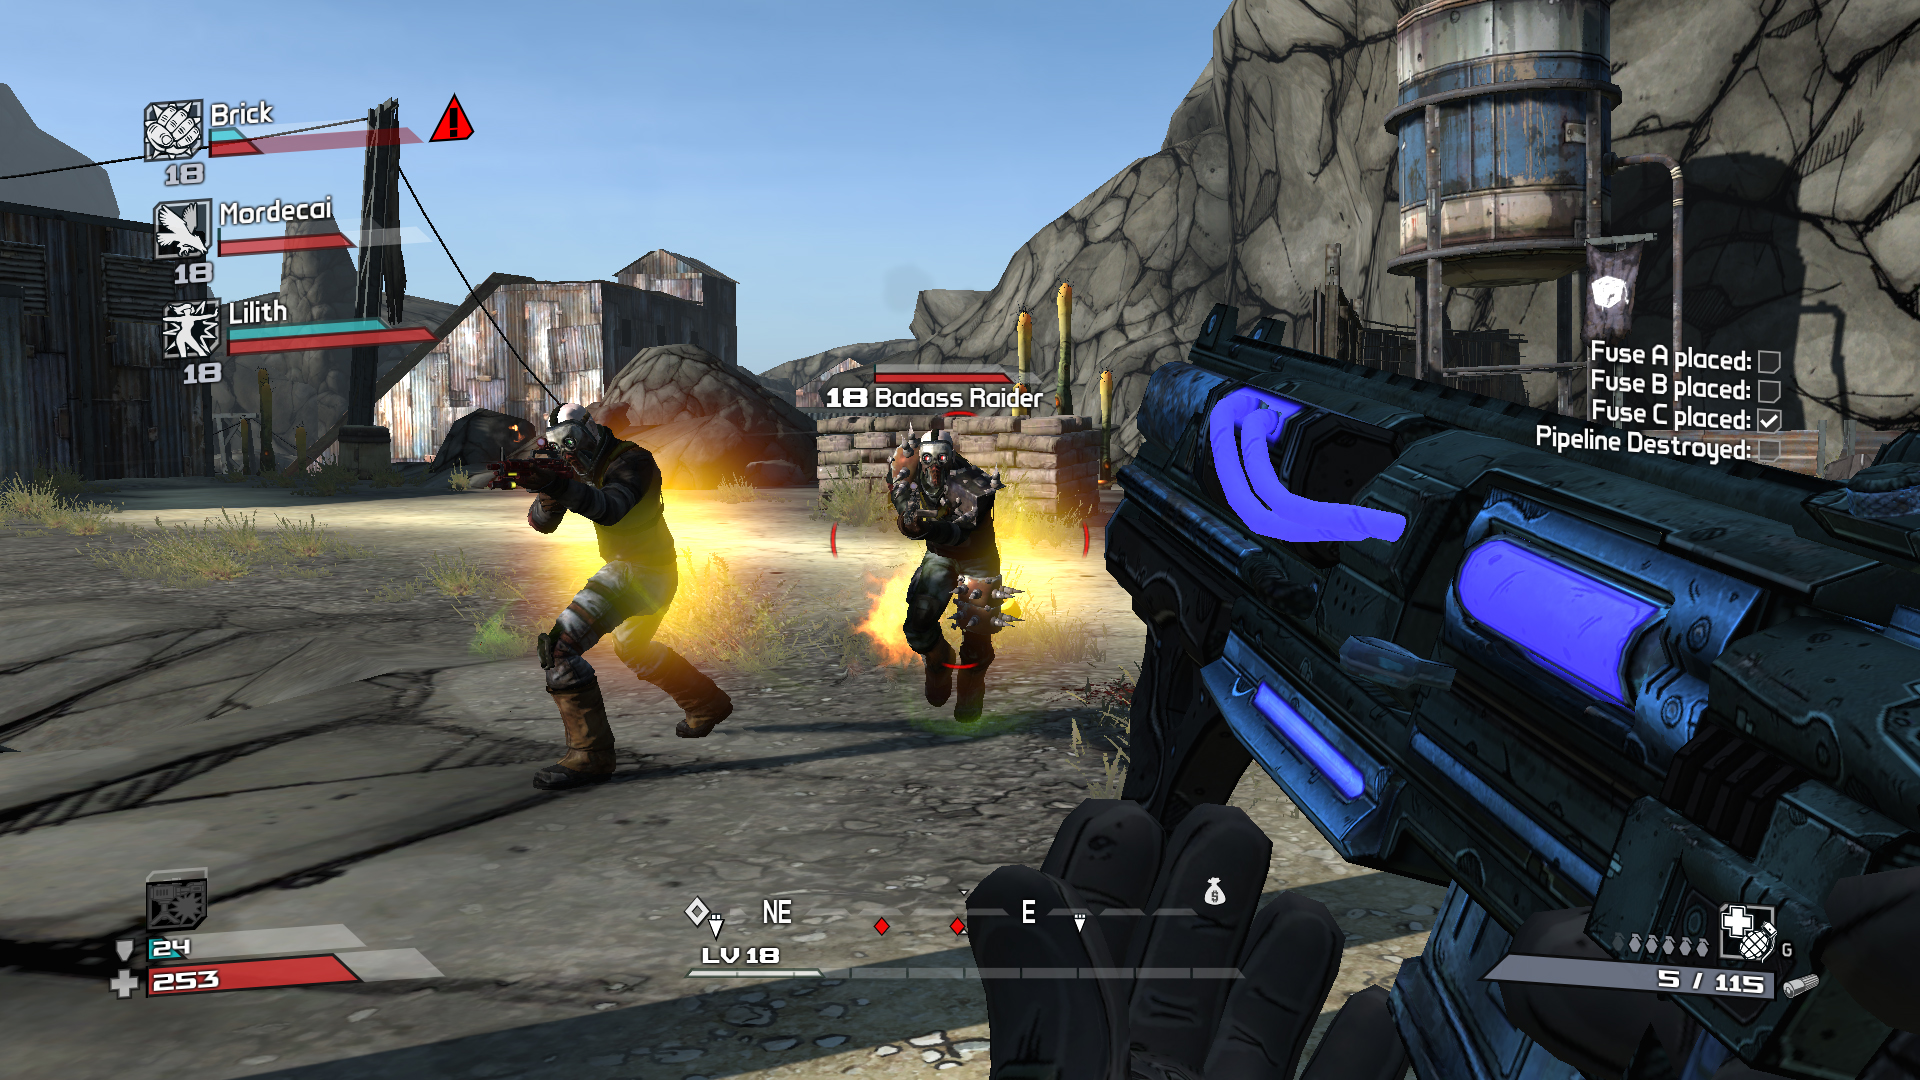
\includegraphics[width=0.8\textwidth]{Imagens/game_borderlands.jpg}
		\caption{Captura de tela do jogo \emph{Borderlands} \cite{game:borderlands}. Tecnicas de \emph{online} PCG foram utilizadas para geração de armas do jogo, produzindo mais de 3 milhões de combinações possíveis.}
		\label{fig:game_borderlands}
	\end{center}
\end{figure}

O controle sobre os efeitos do conteúdo gerado em PCG é tão complexo que vários estudos têm sido realizados na área. Uma nova ramificação de PCG, que se dedica a considerar as experiências de um ator humano para a geração de conteúdo, chamada Geração Procedural de Conteúdo Dirigida à Experiência (\emph{Experience-Driven Procedural Content Generation} - EDPCG), é estudada e detalhada em \cite{yannakakis2011experience}. Na EDPCG, um ator humano (jogador) participa na seleção e evolução de novos conteúdos de forma direta ou indireta, desta forma o conteúdo gerado de forma online pode ser personalizado à cada indivíduo, suprindo suas preferências ou necessidades com base nos dados coletados sobre o mesmo. \cite{hastings2009evolving} e \cite{hastings2009automatic} utilizam um algoritmo evolutivo que se baseia nas preferências do jogador para evoluir diferentes tipos de armas em um jogo de ação e combate de aeronaves.

Como técnicas de \emph{online} PCG são integradas e aplicadas durante a execução dos programas, alguns requisitos se fazem necessários na maioria dos casos: o algoritmo precisa ser executado de forma rápida, necessita ter um tempo de execução previsível e seus resultados devem ter qualidade esperada. Os dois primeiros requisitos, ambos relacionados ao tempo de execução do algoritmo, se devem ao fato de que o uso da \emph{online} PCG muitas vezes ocorre durante a ação do jogo. Em jogos que exigem reflexos rápidos e precisos, gargalos de processamento são inaceitáveis, exigindo que tais técnicas sejam processadas de forma rápida e eficiente. Mesmo quando a PCG é utilizada em fases preparatórias, como em telas de carregamento entre níveis, embora seja aceitável por parte dos usuários aguardar algum tempo, uma espera muito grande se torna algo indesejável e incômodo, afetando inclusive a imersão do jogador no contexto do jogo.

Quanto a qualidade do conteúdo gerado, o problema surge quando alguns itens são criados de forma incompatível ou defeituosa. Enquanto alguns jogos como \emph{Spelunky} \cite{game:spelunky} (Figura \ref{fig:game_spelunky}) se beneficiam pela geração de conteúdos incrivelmente difíceis, a alta dificuldade nestes casos é constante e faz parte de seu \emph{design}; embora sejam extremamente complicados, todos os níveis possuem solução, nenhum conteúdo difícil é gerado por acaso, e a alta dificuldade por consequência do uso de \emph{online} PCG é proposital. Em contraste, conteúdos mal formados podem influenciar a dinâmica do jogo de forma muito negativa. Se algum desafio gerado se torna impossível, ou há um grande declive entre os níveis de desafios gerados, o equilíbrio entre desafio e tédio é rompido e o jogo deixa de ser divertido.

\begin{figure}[htb]
	\begin{center}
		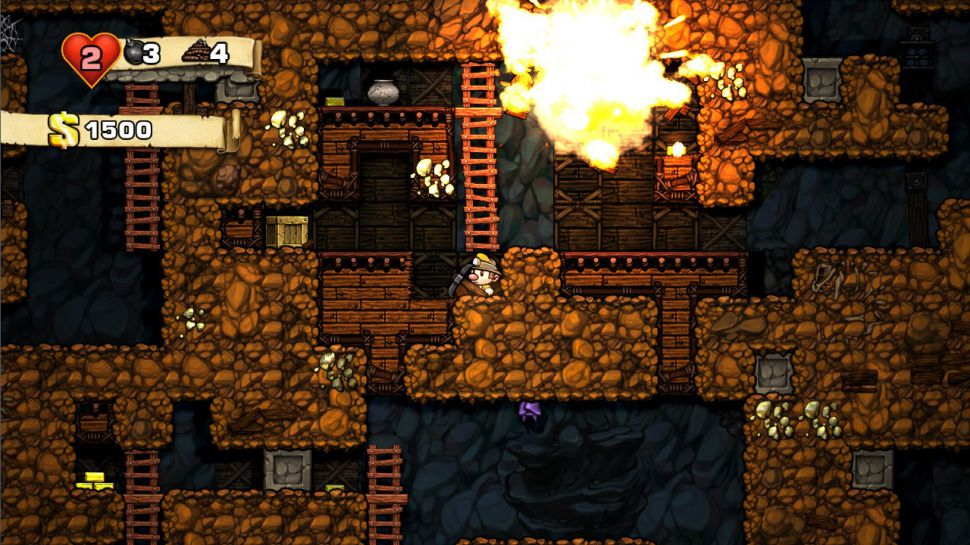
\includegraphics[width=0.8\textwidth]{Imagens/game_spelunky.jpg}
		\caption{Captura de tela do jogo \emph{Spelunky} \cite{game:spelunky}.}
		\label{fig:game_spelunky}
	\end{center}
\end{figure}

Diversas formas de controle de qualidade de conteúdo gerado tem sido estudadas, \cite{togelius2011search} provê um estudo e taxonomia de pesquisas que utilizam algoritmos evolucionários e outras formas meta-heurísticas de algoritmos de busca para gerar conteúdos automaticamente em jogos, dando o nome a estes de Geração Procedural de Conteúdo Baseada em Busca (\emph{Search-Based Procedural Content Generation} - SBPCG). A utilização de Algoritmos Genéticos para controle de qualidade de conteúdo é uma boa solução, mas pode apresentar alguns problemas em relação ao tempo de execução e à diversificação do conteúdo gerado. Dependendo da forma como o problema é modelado, e da natureza do espaço de busca, execuções podem levar um bom tempo para encontrar uma solução satisfatória. Além disso, normalmente os indivíduos obtidos na população final são muito semelhante, e não há garantia de que uma nova execução não irá convergir para o mesmo ponto. Isso pode resultar na falha em obtenção de conteúdo suficientemente diversificado, o que normalmente é uma das principais motivações para o uso de PCG nos jogos de hoje.

Analisando estes problemas, seria interessante um método que consiga gerar, em uma só execução, conteúdo bom e diversificado, garantindo pelo menos um mínimo de qualidade funcional e diferenciação entre si. Tal método poderia ser utilizado tanto de forma \emph{offline}, oferecendo ao desenvolvedor diversas possibilidades de \emph{design} para serem trabalhadas em cima; como de forma \emph{online} em fases preparatórias do jogo, como telas de carregamento, gerando de uma só vez vários itens para serem utilizados durante a execução. Todas estas qualidades em um só método poderiam não só garantir que o jogador não fique entediado e frustrado, como poupar tempo com execuções desnecessárias gerando conteúdos semelhantes e não funcionais. Fora do contexto de jogos, este método poderia ser de excelente aplicação em problemas de auxílio à tomada de decisão onde há a necessidade de sugestões diferenciadas.

\section{Objetivos}

O objetivo geral deste trabalho é a elaboração de uma solução evolutiva que seja capaz de obter um número razoável de indivíduos diferenciados, com qualidade funcional aceitável. Além disso é desejável que esta seja livre de interação humana e que possa ser utilizada tanto de forma \emph{online} quanto \emph{offline}. O contexto utilizado para desenvolvimento e testes será a geração procedural de fases para um jogo de aventura, onde é desejável encontrar mapas visualmente distintos e que possuam uma boa qualidade de navegação e exploração.

Sendo assim, este trabalho propõe o desenvolvimento de uma metodologia que evolua soluções distintas e de qualidade aceitável para sistemas com necessidade de resultados diferenciados.

Os objetivos específicos são:

\vspace{-5mm}
\begin{itemize}[leftmargin=1.25\parindent]
    \item Elaborar a estrutura genética para a construção e evolução de mapas;
    \item Avaliar a qualidade funcional dos mapas através de uma função de avaliação;
    \item Classificar o nível de diferença entre mapas;
    \item Utilizar as qualidades funcionais obtida pelo Algoritmo Genético (AG) convencional;
    \item Utilizar as qualidades de diversidade introduzidas pela Busca Inovativa (\emph{Novelty Search} - NS);
    \item Combinar de forma eficiente as qualidades oferecidas pelo AG convencional e pela NS;
    \item Obter uma quantidade satisfatória de soluções em uma única execução;
    \item Garantir que as soluções encontradas sejam abrangentes e aptas para a solução do problema.
\end{itemize}

\section{Revisão Bibliográfica}

Nesta seção estão apresentados trabalhos que tentam solucionar de diversas maneiras o problema identificando, avaliando seus pontos negativos e positivos. Serão apresentados ainda, trabalhos que possam servir como base ou inspiração para o desenvolvimento da solução ou contexto escolhido.

%kerssemakers2012procedural
A identificação da semelhança de conteúdos gerados de forma automática, \cite{kerssemakers2012procedural} sugere a criação  de um gerador procedural de geradores procedurais para fases de \emph{Super Mario Bros.} \cite{game:mario}, na tentativa de automatizar o processo de variabilidade de conteúdo. Os geradores procedurais finais produzidos pelas técnicas utilizadas, são capazes de evoluir mapas com tema visual comum, sendo facilmente possível identificar as semelhanças entre mapas criados por um mesmo gerador procedural. A Figura \ref{fig:kerssemakers2012procedural} mostra a tela inicial de quatro níveis distintos criados por um mesmo gerador procedural. A proposta do autor é criar, de forma procedural, geradores procedurais com temas visuais diversos, sendo então capaz de usar diferentes geradores resultantes do processo evolutivo para gerar mapas 
distintos.

\begin{figure}[htb]
	\begin{center}
		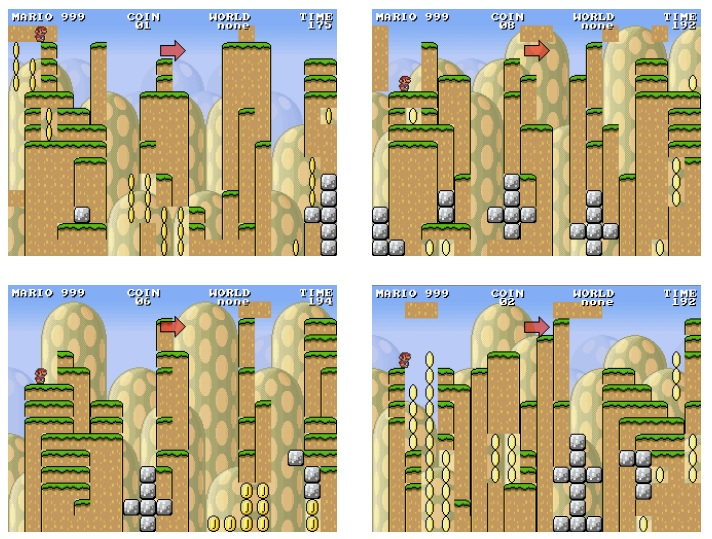
\includegraphics[width=0.8\textwidth]{Imagens/kerssemakers2012procedural.jpg}
		\caption{A tela inicial de quatro níveis distintos criados por um mesmo gerador procedural em \cite{kerssemakers2012procedural}.}
		\label{fig:kerssemakers2012procedural}
	\end{center}
\end{figure}

Com isso, é proposto a criação automática de geradores procedurais distintos com base em SBPCG e EDPCG. Neste processo, geradores procedurais são apresentados a um agente humano, que decide quais geradores serão combinados para formar os indivíduos da próxima geração. Com o resultado final, é possível se criar conjuntos de fases com temas distintos, podendo ser caracterizados como fases de “mundos” diferentes no universo de \emph{Super Mario Bros.}.

Mesmo sendo capaz de gerar fases distintas, a solução se baseia no uso de um ator humano como principal fator de seleção. Por conta disso, este procedimento se torna inviável como solução para o problema proposto, pois é desejável uma solução que possa ser utilizada tanto de forma \emph{offline} como \emph{online}, sem que a imersão do jogador seja quebrada. Além disso, mesmo que o ator humano seja substituído por um agente automatizado, o método não oferece nenhuma garantia de qualidade sobre o conteúdo gerado.

%hastings2009evolving, hastings2009automatic
Em \cite{hastings2009evolving} e \cite{hastings2009automatic} são evoluídas diferentes armas com base nas preferências do jogador para um jogo de combate multi-jogador. A solução é capaz de gerar armas com efeitos visuais incrivelmente diferentes e foi utilizada comercialmente para o lançamento do jogo \emph{Galactic Arms Race} \cite{game:galacticarmsrace}. A Figura \ref{fig:hastings2009evolving} apresenta exemplos de armas geradas para o jogo \emph{Galactic Arms Race} durante uma partida.

\begin{figure}[htb]
	\begin{center}
		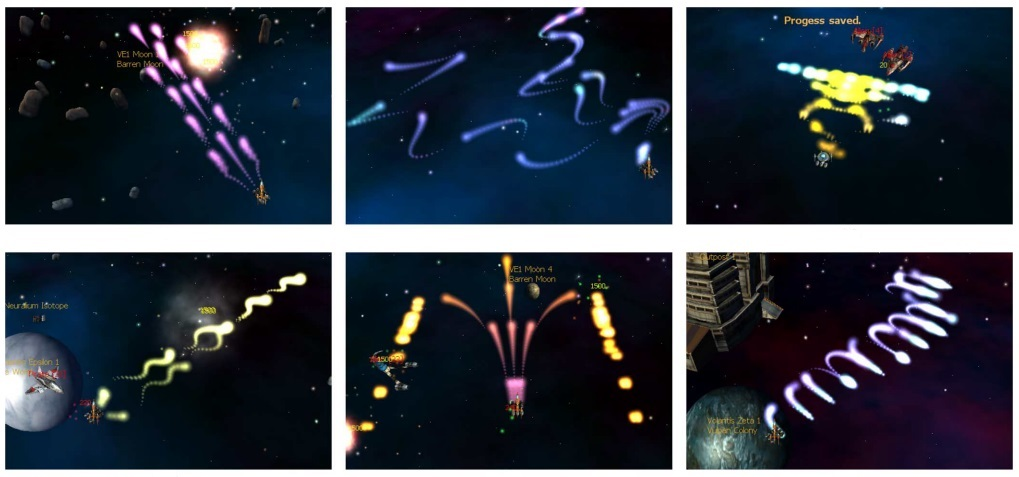
\includegraphics[width=0.8\textwidth]{Imagens/hastings2009automatic.jpg}
		\caption{Exemplos de armas criadas para o jogo \emph{Galactic Arms Race} com a técnica descrita em \cite{hastings2009evolving}.}
		\label{fig:hastings2009evolving}
	\end{center}
\end{figure}

A solução proposta aqui também é uma mistura entre SBPCG e EDPCG, onde partículas visuais para os efeitos da armas são evoluídos com base em um algoritmo evolutivo e em escolhas e preferências dos jogadores. Durante a execução do jogo, cada item recebe uma nota de avaliação baseada na frequência em que aquele conteúdo é efetivamente utilizado. Novos itens são posicionados na fase para que os jogadores possam pegá-los, somente itens apanhados pelo jogador são elegíveis para reprodução. O algoritmo seleciona itens, dentre os já utilizados pelo jogador, para reprodução e geração de novos conteúdos. Os itens são selecionados de forma probabilística com base na nota de avaliação calculada. Para cada novo item adicionado à fase, há uma chance de que um item pré-desenvolvido seja sorteado, garantindo assim um pouco de diversidade e boa qualidade dos itens gerados.

A forma como o jogador contribui para o processo evolutivo é feito de forma inconsciente, sem que isso afete sua imersão em relação ao ambiente criado pelo jogo. Porém, da mesma forma que \cite{kerssemakers2012procedural}, embora o processo consiga evoluir armas incrivelmente diferentes, este se baseia fortemente na necessidade de um ator humano para a seleção de novos conteúdo. Além disso, o processo desenvolvido só é válido para utilização \emph{online} e ativa, excluindo qualquer possibilidade de utilização em etapas de desenvolvimento.

%cardamone2011interactive
Também utilizando uma combinação de SBPCG e EDPCG, \cite{cardamone2011interactive} sugere um processo onde ferramentas separadas são utilizadas para a evolução de pistas para um jogo de corrida. Sua intenção é evoluir pistas que sejam interessantes aos jogadores, avaliando de forma coletiva as melhores pistas geradas pelo sistema. A proposta utiliza uma interface \emph{web} onde jogadores avaliam de forma coletiva quais são as suas pistas favoritas. Um sistema evolutivo utiliza os dados obtidos pela plataforma web para a geração de novas pistas, que ficam então disponíveis dentro do jogo e também passam a ser avaliadas pelos jogadores através da interface \emph{web}. Embora baseado em EDPCG, este processo pode ser visto como completamente \emph{offline}, uma vez que tanto a avaliação como a geração de novos conteúdos é efetuada fora do jogo.

De acordo com os resultados apresentados, a metodologia conseguiu obter melhorias na satisfação dos usuários em relação ao conteúdo gerado. Um problema encontrado entretanto, foi a presença de pistas muito semelhantes a pistas já existentes sendo adicionadas ao sistema. Com isso, as metodologias propostas em \cite{cardamone2011interactive} não são cabíveis ao problema aqui apresentado; não sendo possível de ser aplicado de forma \emph{online}, tendo a necessidade de atores humanos e constantemente gerando conteúdo similar.

%risi2012combining
De forma similar, \cite{risi2012combining} cria uma forma de EDPCG que utiliza redes sociais em conjunto com SBPCG para gerar uma forma de evolução colaborativa entre os jogadores. Sendo a evolução de novas flores parte principal da mecânica do jogo modelo utilizado, munido de um mercado virtual interno, esta técnica gera uma dinâmica de colaboração entre os jogadores em prol da procura de novos conteúdos diferenciados. Sementes são comercializadas entre os jogadores em um mercado global utilizando uma moeda virtual, como consequências de oferta e demanda do mercado, um grande incentivo em busca de novas flores é criado. A Figura \ref{fig:risi2012combining} apresenta um exemplo de flores geradas com fractais através do processo colaborativo de jogadores.

\begin{figure}[htb]
	\begin{center}
		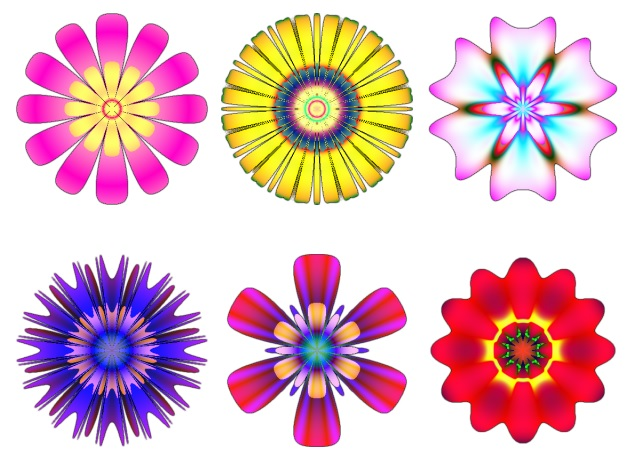
\includegraphics[width=0.6\textwidth]{Imagens/risi2012combining.jpg}
		\caption{Exemplos de flores criadas com fractais através do processo colaborativo de jogadores em \cite{risi2012combining}.}
		\label{fig:risi2012combining}
	\end{center}
\end{figure}

Mesmo sendo capaz de influenciar fortemente a evolução de conteúdo diversificado através de mecânicas de oferta e demanda, assim como o mercado real, a metodologia proposta depende fortemente de uma comunidade ampla para seu funcionamento. Com isso a aplicação de tal técnica se torna inviável para problemas onde a solução deve ser imediata, não sendo efetiva para o objetivo proposto nesta pesquisa.

%liapis2013generating, liapis2013adaptive
O estudo em \cite{liapis2013generating} evolui abstrações de mapas utilizados em jogos de estratégia em tempo real de sucesso como \emph{Starcraft} \cite{game:starcraft}. O método proposto é uma solução completamente \emph{offline}, que otimiza rascunhos de mapas gerados por humanos ou agentes artificiais através de um algoritmo de busca.

Nesta solução, mapas possuem um genótipo codificado que podem representar mapas não jogáveis. Devido a isso, um algoritmo genético com duas populações, uma com indivíduos viáveis e outra com indivíduos inviáveis, são mantidas e evoluídas separadamente. Indivíduos são atribuídos à devida população assim que gerados dependendo do seu estado: viável ou inviável. O estudo também analisa o uso de diferentes funções de avaliação e o uso de uma ou múltiplas funções como nota de avaliação final, demonstrando que o uso de várias funções limitam a eficiência da otimização, mas tendem a obter mapas mais apropriados para uso. A Figura \ref{fig:liapis2013generating} mostra exemplos de mapas evoluídos com o uso de diferentes funções de avaliação.

\begin{figure}[htb]
	\begin{center}
		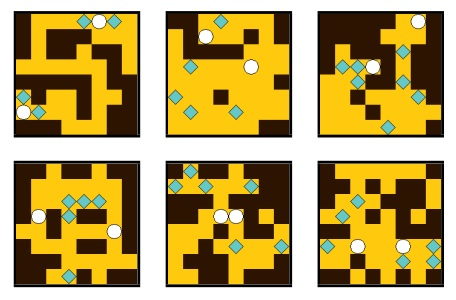
\includegraphics[width=0.6\textwidth]{Imagens/liapis2013generating.jpg}
		\caption{Exemplos de mapas evoluídos com o uso de diferentes funções de avaliação em \cite{liapis2013generating}.}
		\label{fig:liapis2013generating}
	\end{center}
\end{figure}

Dando continuidade ao trabalho desenvolvido em \cite{liapis2013generating}, \cite{liapis2013adaptive} adiciona a interação humana ao processo de evolução. Atores humanos passam a controlar o peso das diversas dimensões da função de avaliação através de um sistema de classificação baseado em preferência pessoal. Os resultados mostram que a técnica introduzida fornece mais controle e converge conteúdos mais rapidamente em direção à real preferência dos usuários se comparado com outras técnicas previamente estudadas.

Embora não tenham foco em diversificação de conteúdo gerado, tais estudos mostram a importância da decisão da função de avaliação para a evolução de conteúdos como mapas para jogos. Diversos aspectos podem ser considerados, podendo ter grande influência nos resultados finais. Além disso, uma reflexão sobre conteúdos viáveis e inviáveis é aberta e pode ajudar no processo de decisão de representação genotípica e fenotípica dos itens gerados.

%lehman2008exploiting, lehman2011abandoning
Em contraste aos algoritmos genéticos convencionais, o algoritmo de Busca Inovativa (\emph{Novelty Search} - NS), introduzido e detalhado em \cite{lehman2008exploiting} e \cite{lehman2011abandoning}, vem sido utilizado em diversos problemas de busca por inovação. Embora tenha sido desenvolvido para auxílio em soluções de problemas combinatórios que confundem a solução, as características divergentes da NS beneficiam muito a busca por novos contextos.

A NS utiliza um cálculo de dispersão, normalmente baseado em uma função de distância comportamental, para classificar o nível de inovação dos indivíduos da população em cada geração. Indivíduos recebem notas baseadas em quão esparsos são as regiões em que se encontram; indivíduos em regiões muito esparsas recebem altas notas inovação, enquanto indivíduos em regiões densas recebem baixas notas de inovação. Um arquivo de indivíduos inovadores é mantido; sempre que um indivíduo recebe uma alta nota de inovação, ele é adicionado permanentemente ao arquivo, que por sua vez também é utilizado para o cálculo de dispersão em todas as gerações. Desta forma a NS mantém uma busca por inovação baseada no tipo de função de distância definido, o arquivo permanente de indivíduos inovadores ajuda a manter um histórico de onde a busca já esteve e incentiva novas regiões a serem exploradas.

Por ser uma busca divergente, o uso da NS pode auxiliar na busca por conteúdo diversificado, não ficando concentrada em regiões de máximo ou mínimo local como algoritmos genéticos convencionais.

%cuccu2011novelty
O sucesso do uso da NS em problemas de otimização, entretanto, está fortemente conectado à definição da função de inovação. Além disso,  \cite{cuccu2011novelty} mostra que em problemas onde o espaço de busca é muito grande, a NS sozinha não é capaz de superar os resultados obtidos pelo Algoritmo Genético convencional. \cite{cuccu2011novelty} demonstra também que uma combinação entre a busca por diversidade e busca por performance convencional pode melhorar muito os resultados obtidos dependendo do problema estudado.

A seguir são apresentados alguns exemplos onde a NS tem sido aplicada com sucesso para a evolução de conteúdo diversificado.

%liapis2015constrained, liapis2013enhancements
Extendendo o trabalho realizado em \cite{liapis2013generating} e \cite{liapis2013adaptive}, \cite{liapis2015constrained} e \cite{liapis2013enhancements} adicionam o conceito de NS ao algoritmo de duas populações para a evolução de conteúdo viável em um jogo de estratégia em tempo real.

De forma similar, as soluções propostas que utilizam a NS também mantém duas populações separadas, uma com indivíduos viáveis e outra com indivíduos inviáveis. Estas possuem restrições de troca genética entre si e novos indivíduos são atribuídos às suas devidas populações com base em sua viabilidade. Duas soluções utilizando a NS são propostas: na primeira, a população inviável utiliza a NS para minimizar a distância entre seus indivíduos e os indivíduos da população viável, enquanto a população viável utiliza a NS para maximizar a inovação; na segunda proposta, a NS é utilizada para maximizar a inovação em ambas as populações.

Os resultados obtidos pelo autor mostram que a primeira configuração é capaz de convergir resultados satisfatórios mais rapidamente que os métodos previamente estudados, enquanto a segunda configuração é capaz de obter uma maior diversidade de soluções finais. Tais resultados são interessantes pois mostram que as características de busca por diversidade introduzidos pela NS podem ser utilizada de forma diferente da proposta originalmente e ainda obter bons resultados diversificados. A utilização de populações viáveis e inviáveis, contudo, é uma situação que pode ser evitada na elaboração da representação genotípica e fenotípica do problema.

%liapis2013sentient
Em \cite{liapis2013sentient} é introduzida uma técnica que combina procura pelo gradiente, através de \emph{backpropagation}, e NS para criação de uma ferramenta de auxílio e melhoria de criatividade humana, oferecendo formas para se refinar rascunhos de terrenos gerados adicionando detalhes e dissimilaridades entre soluções.

A NS é utilizada para gerar redes neurais artificiais dissimilares, que são treinadas para se aproximarem de um rascunho apresentado, e então providenciar mapas com maiores níveis de detalhe. Em processos iterativos, os resultado são apresentados à um ator humano, que rejeita, aceita ou altera as soluções apresentadas, e então continuam a evoluir mais detalhes até formar mapas completos com alta resolução, podendo ou não divergir do rascunho inicial oferecido para o treinamento. A Figura \ref{fig:liapis2013sentient} apresenta a interface utilizada pelo ator para escolher um mapa de maior resolução para prosseguir. A ferramenta dá suporte ao processo criativo do ator humano, oferecendo variações da proposta inicial apresentada, enquanto o mantém em controle sobre o conteúdo sendo evoluído durante todo o processo através das etapas iterativas. Os resultados obtidos mostram que o uso da NS é benéfico para a obtenção de conteúdos divergentes sem reduzir a velocidade de refinamento iterativo dos mapas.

\begin{figure}[htb]
	\begin{center}
		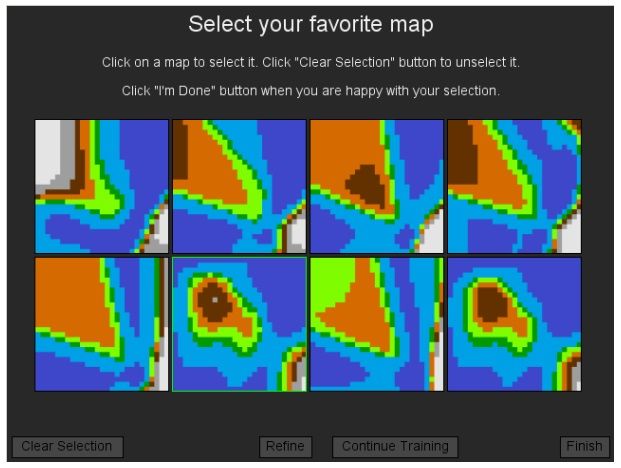
\includegraphics[width=0.6\textwidth]{Imagens/liapis2013sentient.jpg}
		\caption{Tela de seleção da ferramenta implementada em \cite{liapis2013sentient} onde o ator escolhe um mapa de maior resolução para prosseguir.}
		\label{fig:liapis2013sentient}
	\end{center}
\end{figure}

%woolley2014novel
Também utilizando uma combinação de processos com interatividade humana e NS, \cite{woolley2014novel} evolui comportamentos de navegação para robôs em um labirinto complexo. A solução permite que um ator humano escolha não só os parâmetros de evolução entre cada iteração, como também permite que ele escolha qual método será usado para as próximas iterações e quais indivíduos devem ser evoluídos através da NS. A combinação da intuição humana em encontrar comportamentos que sejam capazes de solucionar o problema, com a capacidade de diversificar as opções sendo oferecidas quando desejado contribuem para uma convergência mais rápida em direção a solução. Os resultados obtidos mostram que a taxa de qualidade da evolução é acelerada e a fatiga do ator humano é reduzida significativamente.

As técnicas apresentadas tanto em \cite{liapis2013sentient} quanto em \cite{woolley2014novel}, são técnicas estritamente \emph{offline} que necessitam da intuição de um ator humano para seu funcionamento. Avaliando estas e outras técnicas com base em interação humana previamente apresentadas, podemos concluir que qualquer solução baseada em EDPCG não é satisfatória para a resolução do problema aqui proposto. Quando dependente de um ator humano, a solução se torna dependente de contexto e normalmente é restrita a funcionamento somente \emph{online} ou somente \emph{offline}. Deseja-se uma solução que seja livre da necessidade de interação humana e que seja capaz de separar diferentes soluções de forma rápida e eficiente, garantindo a diversidade e qualidade dos itens gerados.

%lehman2011evolving
Neste sentido, a solução proposta em \cite{lehman2011evolving} se aproxima perfeitamente do objetivo geral desta pesquisa, sendo capaz de evoluir soluções distintas sem a necessidade de atores humanos. \cite{lehman2011evolving} sugere a combinação da função de avaliação convencional com a função de inovação proposta pela NS, através de um algoritmo com otimização baseado em eficiência à Pareto, para a evolução de criaturas virtuais com capacidade de locomoção. A Figura \ref{fig:lehman2011evolving} apresenta um exemplo de criaturas virtuais com capacidade de locomoção razoável e diferentes morfologias encontradas em uma única execução do algoritmo.

\begin{figure}[htb]
	\begin{center}
		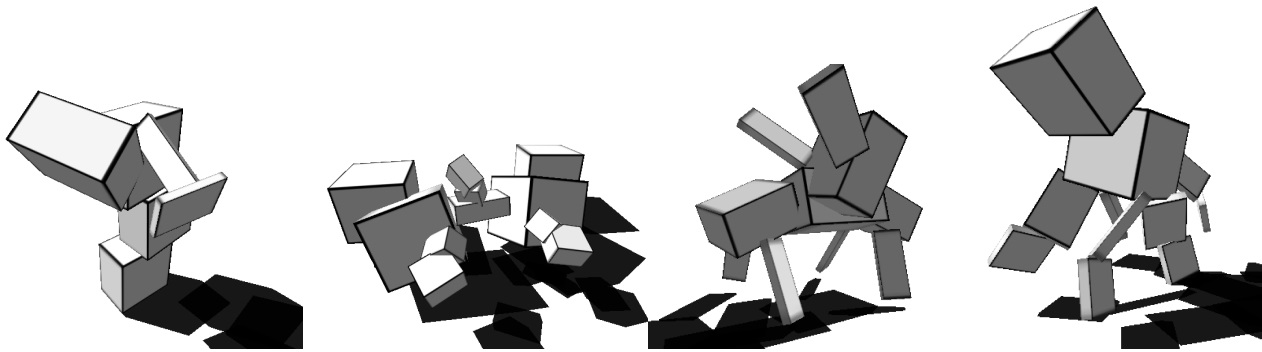
\includegraphics[width=0.8\textwidth]{Imagens/lehman2011evolving.jpg}
		\caption{Exemplo de criaturas virtuais com capacidade de locomoção razoável e diferentes morfologias encontradas em uma única execução do algoritmo apresentado em \cite{lehman2011evolving}.}
		\label{fig:lehman2011evolving}
	\end{center}
\end{figure}

O algoritmo utilizado em questão é o NSGA-II, um algoritmo evolutivo multi-objetivo com eficiência à Pareto proposto e detalhado em \cite{deb2002fast}. Além da combinação entre performance e inovação, a solução propõe a utilização de uma métrica de Nota Local, que quando combinada à métrica de inovação em um algoritmo de eficiência à Pareto é capaz de manter nichos morfológicos durante toda a busca. Nichos morfológicos são regiões que possuem similaridades no espaço das morfologias, este gerado pela função de distância definida para o algoritmo de NS. Diferentes nichos morfológicos possuem diferentes capacidades funcionais, a solução utilizada se mostra capaz de explorar eficientemente cada nicho, obtendo os melhores indivíduos em cada um deles.

Embora utilizada para evoluir criaturas virtuais com capacidade de locomoção, se bem elaborada, a solução pode ser aplicada no contexto de evolução de mapas para jogos de exploração e aventura. A solução porém, explora todos os nichos morfológicos existentes, mantendo indivíduos de nichos tanto de alta como baixa capacidade.

%lehman2010revising,  gomes2012progressive
O conceito de critério mínimo para a NS é introduzido em \cite{lehman2010revising} e depois elaborado de forma mais genérica em  \cite{gomes2012progressive}, sem a necessidade de parâmetros iniciais dependentes de contexto.

A ideia por trás do critério mínimo é que indivíduos precisam atingir uma capacidade funcional mínima aceitável para que sejam elegíveis para reprodução. Desta forma, qualquer indivíduo da população que não tenha atingido um valor funcional mínimo em relação a função de avaliação, é atribuído a uma nota zero de inovação, sendo escolhidos para reprodução somente caso todos os outros indivíduos restantes tenham nota zero de inovação. Desta forma, a NS exclui, ou minimiza, a quantidade de indivíduos "ruins"~durante o processo evolutivo, e a exploração, embora continue divergente, tende a navegar em áreas com melhores capacidades funcionais.

Os resultados obtidos mostram que, especialmente a versão de critério mínimo proposta em \cite{gomes2012progressive}, é capaz de superar outras configurações utilizando somente Algoritmo Genético e NS, especialmente em problemas com o de labirintos de difícil navegação. O uso de um critério mínimo pode auxiliar na obtenção de indivíduos com melhor capacidade funcional ao mesmo tempo que permite que a NS busque por inovação.

%mapas
A seguir são apresentados alguns trabalhos onde o principal contexto é a geração procedural de mapas, mesmo não havendo foco em diversidade nos resultados obtidos. São estudadas principalmente as formas de representação e avaliação de mapas, visando buscar inspiração e conceitos para aplicação nesta pesquisa.

%van2014procedural
Em \cite{van2014procedural} é apresentado um estudo específico sobre métodos de PCG para mapas de jogos de aventura. Ele resume práticas comuns, discute prós e contras de diferentes técnicas e identifica desafios promissores. O estudo descreve as técnicas atuais como boas em performance, mas deficientes em relação à controle e precisão sobre o conteúdo gerado.

Em geral, técnicas de PCG para criação de mapas consistem em três elementos: um modelo representativo, um método para montar o modelo representativo e um método para criar a geometria real do mapa com base em um modelo representativo qualquer. O estudo detalha métodos que são relevantes a técnicas de PCG e os classifica em autômatos celulares, gramáticas generativas, algoritmos genéticos e baseados em restrições. As análises sobre as técnicas de PCG baseadas em algoritmo genético revelam diversas formas interessantes de representação genotípica e fenotípica para os mapas. Também são estudadas diversas formas de gerar a função de avaliação, detalhando as vantagens e desvantagens de cada uma delas.

O estudo revela que várias técnicas presentes são capazes de gerar diversos tipos de representações finais e todas dependem do contexto e intenção do conteúdo gerado. As técnicas em geral são rápidas o suficiente, mesmo o contexto onde são aplicadas não requerendo uma resposta imediata, com os mapas sendo gerados durante telas de carregamento ou em segundo plano enquanto o jogador já está em jogo para gerar os próximos níveis.

%ashlock2011search
Em um estudo mais específico, \cite{ashlock2011search} propõe diferentes formas de representação de mapas e formas de avaliação do conteúdo gerado. Foco é dado para mapas que tenham uma estrutura parecida com a de um labirinto, tornando a exploração um dos principais focos do conteúdo gerado.

Quatro principais formas de representação são sugeridas e estudadas: direta, cromática, positiva e negativa. Em todas as representações o mapa é dividido em forma de grade, e as possíveis entradas em cada setor é aberto ou fechado, com aberto representando lugares onde se pode caminhar e fechado representando paredes ou obstáculos. Na representação direta os blocos abertos e fechados são representados diretamente em um único e longo gene; a representação cromática atribui cores à cada setor para controlar a movimentação de um agente que irá gerar toda a área aberta do mapa; a representação positiva possui em seu gene estruturas que são posicionadas em uma grade completamente aberta, formando diversas paredes e obstáculos; e a representação negativa inicia com um mapa completamente fechado e possui em seu genótipo as estruturas que serão abertas para gerar o mapa, como salas e corredores. A Figura \ref{fig:ashlock2011search} apresenta exemplos de mapas criados pela representações cromática, positiva e negativa. Além das representações e das funções de avaliação definidas, a técnica utiliza de um sistema de \emph{checkpoints} para garantir a conectividade e comprimento dos caminhos dentro de um mapa.

\begin{figure}[htb]
	\begin{center}
		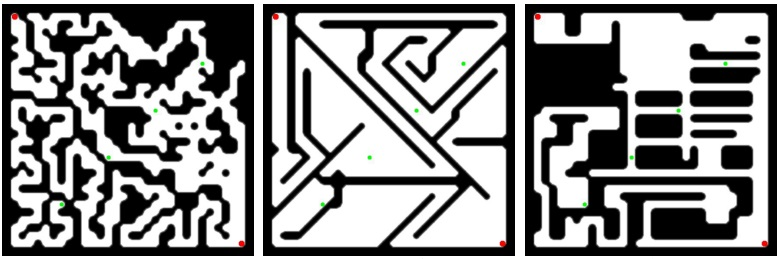
\includegraphics[width=0.8\textwidth]{Imagens/ashlock2011search.jpg}
		\caption{Da esquerda para a direita, exemplos de mapas criados pelas representações cromática, positiva e negativa em \cite{ashlock2011search}.}
		\label{fig:ashlock2011search}
	\end{center}
\end{figure}

O estudo, além de contribuir com diferentes formas de representação e funções de avaliação, mostra que diferentes técnicas podem ser utilizadas com as mesmas funções de avaliação, mas resultam em mapas completamente diferentes. Isso revela que além da função de avaliação, a escolha das técnicas e representações dos mapas pode afetar de forma drástica os resultados obtidos.

%valtchanov2012evolving
Outro estudo interessante, \cite{valtchanov2012evolving}, apresenta uma técnica para representação e evolução de mapas que possuem critérios mais complexos em sua estrutura. Os mapas gerados dão suporte a salas com eventos e regiões separadas por salas únicas, onde geralmente, em jogos de aventura, o jogador é forçado a obter uma chave ou completar algum quebra-cabeça para obter acesso.

O cromossomo utilizado neste método é uma estrutura de árvore onde cada nó representa uma peça a ser posicionada e a porta a ser utilizada para conectar aos seus pais. As peças são pré-definidas em relação a tamanho, forma e posicionamento das portas. Durante o processo de tradução, a árvore é processada iniciando da raiz (sala inicial) e adicionando as salas de seus nós filhos. Novas peças são posicionadas e rotacionadas de forma a se conectar às salas anteriores, caso não seja possível adicionar a nova peça sem gerar colisão entre peças já existentes, o nó que a representa e todos os seus descendentes são removidos do genótipo. A Figura \ref{fig:valtchanov2012evolving} mostra exemplos de mapas gerados através desta técnica.

\begin{figure}[htb]
	\begin{center}
		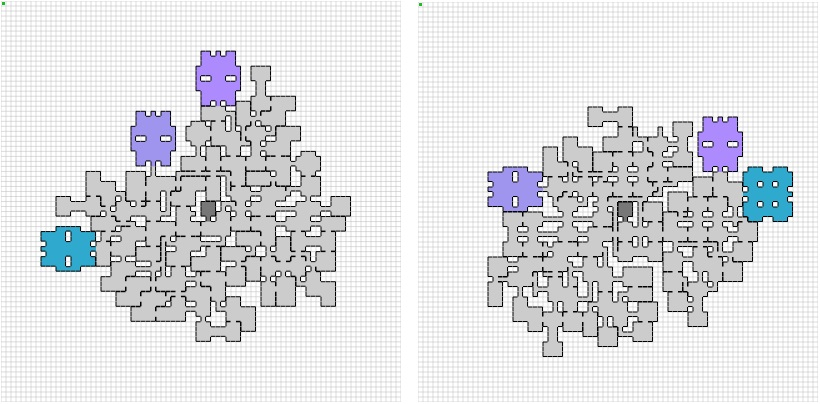
\includegraphics[width=0.8\textwidth]{Imagens/valtchanov2012evolving.jpg}
		\caption{Exemplos de mapas gerados através da técnica proposta em \cite{valtchanov2012evolving}.}
		\label{fig:valtchanov2012evolving}
	\end{center}
\end{figure}

Os mapas resultantes são visualmente interessantes e tendem a possuir boas características para um jogo de aventura e exploração. Porém, foi identificado que com a adição de novas restrições para separações de áreas e salas de evento, surge um grande problema de máximo local, com o algoritmo gerando constantemente soluções muito parecidas.

%cardamone2011evolving
\cite{cardamone2011evolving} estuda formas de utilizar a PCG para criar mapas interessantes para jogos de tiro em primeira pessoa. Em sua solução, são sugeridas quatro formas de representação de mapas, sendo duas baseadas nas formas apresentadas em \cite{ashlock2011search}: a positiva, adicionando paredes e obstáculos à um mapa inicialmente aberto; e a negativa, abrindo corredores e salas em um mapa inicialmente fechado. Das outras duas soluções, uma se baseia em um agente artificial para cavar regiões abertas em um mapa inicialmente fechado, e outra em uma estrutura onde o mapa é subdividido em grades maiores e paredes são removidas formando as conexões entre as áreas. A Figura \ref{fig:cardamone2011evolving} apresenta exemplos de mapas criados pelas diferentes representações propostas.

\begin{figure}[htb]
	\begin{center}
		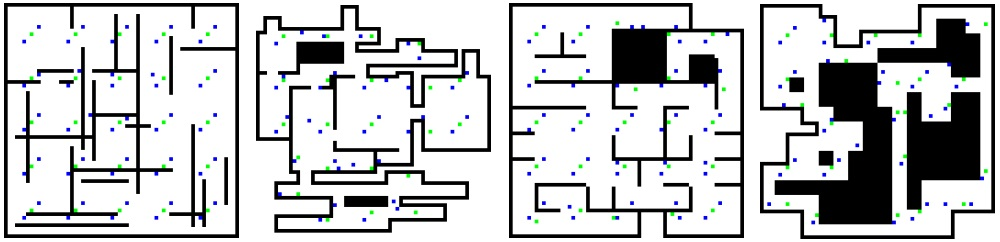
\includegraphics[width=0.8\textwidth]{Imagens/cardamone2011evolving.jpg}
		\caption{Exemplos de mapas criados pelas diferentes representações propostas em \cite{cardamone2011evolving}.}
		\label{fig:cardamone2011evolving}
	\end{center}
\end{figure}

De acordo com o objetivo proposto em \cite{cardamone2011evolving}, as representações com maior potencial foram a positiva e a baseada em grade, pois oferecem maior tempo de combate entre jogadores no ambiente simulado de um jogo de tiro. Em contrapartida \cite{lanzi2014evolving} utiliza a representação negativa para criar mapas balanceados para jogos do mesmo estilo, alegando que os mapas gerados pela representação negativa possuem uma estrutura interessante, com vários corredores e grandes salões. A Figura \ref{fig:lanzi2014evolving} mostra exemplos de mapas gerados em \cite{lanzi2014evolving} utilizando somente a representação negativa.

\begin{figure}[htb]
	\begin{center}
		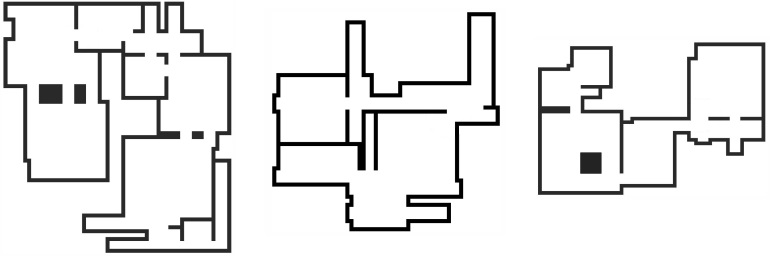
\includegraphics[width=0.8\textwidth]{Imagens/lanzi2014evolving.jpg}
		\caption{Exemplos de mapas gerados em \cite{lanzi2014evolving} que utilizam somente a representação negativa proposta em \cite{cardamone2011evolving}.}
		\label{fig:lanzi2014evolving}
	\end{center}
\end{figure}

Se comparado com a representação negativa apresentada em \cite{ashlock2011search}, a representação sugerida por \cite{cardamone2011evolving}, e utilizada por \cite{lanzi2014evolving}, é mais simples e não necessita do sistema de \emph{checkpoints} para gerar mapas interessantes. Por isso, e por gerar estruturas interessantes, esta representação pode ser interessante para jogos de aventura e exploração.

\section{Estrutura da Dissertação}

Este documento está dividido em cinco capítulos: Introdução, Metodologia, Desenvolvimento, Experimentos e Resultados e Conclusão.

No capítulo Introdução é contextualizado o conceito de PCG, tanto de forma geral, quanto específica em relação à pesquisa, mostrando algumas de suas aplicações no mercado e em pesquisas. Também são apresentados os objetivos definidos e a justificativa da realização do trabalho.

Em Metodologia são detalhadas as principais técnicas e temas pesquisadas e utilizadas como base neste trabalho, abrangendo as áreas de Algoritmos Genéticos, eficiência à Pareto e separação de nichos.

Já no capítulo Desenvolvimento são descritas todas as modificações e técnicas utilizadas para a implementação da solução proposta para o problema.

Em Experimentos e Resultados são explicados os testes que foram executados para a validação do sistema implementado, detalhando os procedimentos seguidos e apresentando com gráficos e tabelas a análise dos comportamentos e valores obtidos.

Por fim, no capítulo Conclusão são considerados os resultados obtidos frente aos objetivos propostos, assim como a indicação de trabalhos futuros para a continuidade da pesquisa.